% fig:cari — CARI training diagram, styled to match fig:architecture.
% Thumbnails from tests/viz/gen_cari_thumbs.py (documents/thesis/images/arch/cari_*.png).
\begin{figure}[t!]
  \centering
  \resizebox{0.96\textwidth}{!}{%
  \begin{tikzpicture}[
      font=\sffamily, >=latex,
      thumb/.style={inner sep=0pt, draw=black!55, line width=0.4pt},
      model/.style={draw=myblue!55, fill=myblue!12, rounded corners=2pt, align=center,
                    minimum width=17mm, minimum height=34mm, line width=0.5pt},
      loss/.style={draw=red!55!black, circle, fill=red!7, inner sep=1pt, minimum size=11mm,
                   font=\small, text=red!60!black},
      io/.style={align=center, font=\small},
      dim/.style={font=\scriptsize\itshape, text=black!55, align=center},
      flow/.style={->, line width=0.8pt, black!70},
    ]

    % ── the cross-illuminant input pair (real, pixel-aligned) ───────
    \node[thumb] (i1) {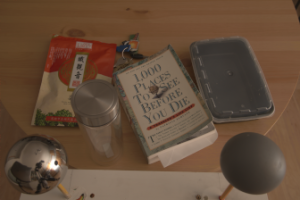
\includegraphics[width=20mm]{images/arch/cari_I1.png}};
    \node[io, above=0.5mm of i1] {$\mathbf{I}_1$ \scriptsize(warm light)};
    \node[thumb, below=12mm of i1] (i2) {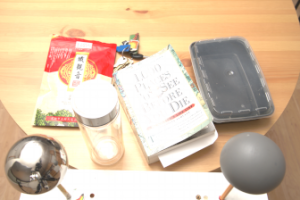
\includegraphics[width=20mm]{images/arch/cari_I2.png}};
    \node[io, below=0.5mm of i2] {$\mathbf{I}_2$ \scriptsize(cool light)};
    \node[dim, below=4mm of i2] {same scene, pixel-aligned,\\raw (\emph{no} white balance)};

    % ── one model, shared weights, two forward passes ──────────────
    \node[model] (m) at ($(i1)!0.5!(i2) + (30mm,0)$) {Model\\[3pt]\emph{shared}\\\emph{weights}\\[3pt]{\scriptsize two forward}\\{\scriptsize passes}};

    % ── predicted albedos (should be identical) + shadings ─────────
    \node[thumb, right=16mm of m.east |- i1] (a1) {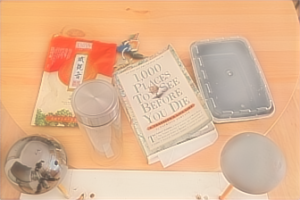
\includegraphics[width=15mm]{images/arch/cari_A1.png}};
    \node[thumb, right=16mm of m.east |- i2] (a2) {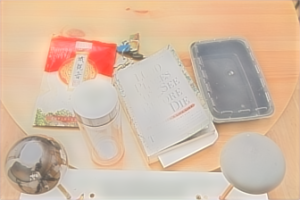
\includegraphics[width=15mm]{images/arch/cari_A2.png}};
    \node[io, above=0.5mm of a1] {$\mathbf{A}_1$}; \node[io, below=0.5mm of a2] {$\mathbf{A}_2$};

    \node[thumb, right=26mm of a1] (s1) {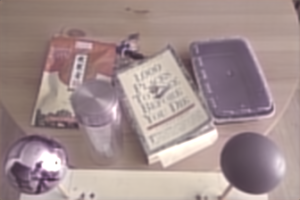
\includegraphics[width=15mm]{images/arch/cari_S1.png}};
    \node[thumb, right=26mm of a2] (s2) {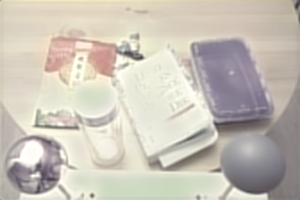
\includegraphics[width=15mm]{images/arch/cari_S2.png}};
    \node[io, above=0.5mm of s1] {$\mathbf{S}_{d,1}$}; \node[io, below=0.5mm of s2] {$\mathbf{S}_{d,2}$};

    % ── flows ──────────────────────────────────────────────────────
    \draw[flow] (i1.east) -- (m.west |- i1);
    \draw[flow] (i2.east) -- (m.west |- i2);
    \draw[flow] (m.east |- a1) -- (a1);
    \draw[flow] (m.east |- a2) -- (a2);
    \draw[flow] (a1.north) to[bend left=18] (s1.north west);
    \draw[flow] (a2.south) to[bend right=18] (s2.south west);

    % ── the two CARI losses ────────────────────────────────────────
    \node[loss] (linv) at ($(a1)!0.5!(a2)$) {$\mathcal{L}_{\text{inv}}$};
    \draw[<->, red!55!black, line width=0.9pt] (a1.south) -- (linv);
    \draw[<->, red!55!black, line width=0.9pt] (a2.north) -- (linv);
    \node[dim, right=0.5mm of linv, text=red!55!black] {$\mathbf{A}_1\!=\!\mathbf{A}_2$\\\scriptsize (material only)};

    \node[loss] (lexp) at ($(s1)!0.5!(s2)$) {$\mathcal{L}_{\text{expl}}$};
    \draw[<->, red!55!black, line width=0.9pt] (s1.south) -- (lexp);
    \draw[<->, red!55!black, line width=0.9pt] (s2.north) -- (lexp);
    \node[dim, right=0.5mm of lexp, text=red!55!black, align=left]
      {$\dfrac{L(\mathbf{S}_{d,1})}{L(\mathbf{S}_{d,2})}\!=\!\dfrac{L(\mathbf{I}_1)}{L(\mathbf{I}_2)}$\\\scriptsize (shading absorbs the cast)};

  \end{tikzpicture}}
  \caption[Cross-Render Albedo Invariance during training.]{%
    Cross-Render Albedo Invariance (CARI), applied only at training time. A pixel-aligned
    pair of the same scene under different coloured illuminants is passed through the
    \emph{same} model (shared weights) in two forward passes. The input thumbnails carry
    visibly different casts, yet the two predicted albedos $\mathbf{A}_1,\mathbf{A}_2$ are
    nearly identical, as enforced by $\mathcal{L}_{\text{inv}}$, while
    the predicted shadings $\mathbf{S}_{d,1},\mathbf{S}_{d,2}$ differ, having absorbed the
    illuminant. $\mathcal{L}_{\text{expl}}$ makes that explicit: it forces the ratio of the
    two shadings to match the ratio of the two inputs, so any colour the albedo declines to
    absorb must be explained by the shading. White balance is disabled for these pairs
    (\secref{sec:raw_pairs}) so that the illuminant colour survives in the input ratio that
    $\mathcal{L}_{\text{expl}}$ reads. Thumbnails are this model's own outputs.
  }
  \label{fig:cari}
\end{figure}
